%!TEX root = forallxdo.tex
\part{Interpretationen}
\label{ch.semantics}
\addtocontents{toc}{\protect\mbox{}\protect\hrulefill\par}


\chapter{Extensionalität}\label{s:Interpretations}

Die WFL ist eine wahrheitsfunktionale Sprache. Ihre Junktoren sind alle wahrheitsfunktional, und alles, was wir mit der WFL tun können, ist, Sätzen bestimmte Wahrheitswerte zuzuweisen. Wir können dies \emph{direkt} tun. Zum Beispiel können wir festlegen, dass der WFL-Satz `$P$' wahr ist. Alternativ können wir dies \emph{indirekt} tun, indem wir einen Symbolisierungsschlüssel anbieten:
	\begin{ekey}
		\item[P] Big Ben ist in London
	\end{ekey}
Wie wir in \S\ref{s:TruthFunctionality} gesagt haben, ist ein Symbolisierungsschlüssel \emph{nur} ein Mittel, um `$P$'s Wahrheitswert festzulegen. Der Symbolisierungsschlüssel besagt ungefähr:
	\begin{ebullet}
		\item Der WFL Satz `$P$' ist wahr gdw Big Ben in London ist.
	\end{ebullet}
Und wir betonten in \S\ref{s:TruthFunctionality}, dass die WFL nicht mit Bedeutungsunterschieden umgehen kann, die über blo{\ss}e Unterschiede im Wahrheitswert hinausgehen. 

\section{Symbolisierung und Übersetzung}
Die LEO hat ähnliche Einschränkungen. Sie geht über blo{\ss}e Wahrheitswerte hinaus, da sie uns ermöglicht, Sätze in Terme, Prädikate und Quantoren zu zerlegen. Dies lässt uns betrachten, was auf ein bestimmtes Objekt, zumindest ein oder alle Objekten zutrifft. \emph{Aber das ist alles}.

Um dies zu erklären, betrachten Sie den folgenden Symbolisierungsschlüssel: 
	\begin{ekey}
		\item[\atom{D}{x}] \gap{x} unterrichtet Logik in Dortmund
	\end{ekey} 
Diese Bestimmung hat nicht zur Folge, dass die \emph{Bedeutung} des deutschen Prädikats mit der des LEO-Prädikats übereinstimmt. Wir schreiben lediglich so etwas vor wie:
	\begin{ebullet}
		\item `$\atom{D}{x}$' und `\gap{x} unterrichtet Logik in Dortmund' treffen auf die gleichen Objekte zu. 
	\end{ebullet}
Also:
	\begin{ebullet}
		\item `$\atom{D}{x}$' trifft auf genau jene Objekte zu, die in Dortmund Logik unterrichten (welche auch immer das sind).
	\end{ebullet}
Dies ist ein \emph{indirekter} Weg, um festzulegen, auf welche Dinge ein Prädikat zutrifft. Alternativ können wir die Objekte, auf die ein Prädikat zutrifft, auch \emph{direkt} festlegen. Zum Beispiel können wir festlegen, dass `$\atom{D}{x}$' auf Simon Wimmer allein zutrifft. Wie es der Zufall will, hätte diese direkte Bestimmung dasselbe Resultat wie die indirekte Bestimmung, da Simon, und nur Simon, in Dortmund Logik unterrichtet. Beachten Sie jedoch, dass die deutschen Prädikate `\blank\ ist Simon Wimmer' und `\blank\ lehrt Logik in Dortmund' sehr unterschiedliche Bedeutungen haben!

Der Punkt ist, dass die LEO keine Ressourcen für den Umgang mit bestimmten Bedeutungsnuancen hat. Wenn wir die LEO interpretieren, dann denken wir nur daran, worauf die Prädikate zutreffen, unabhängig davon, ob wir diese Objekte direkt oder indirekt bestimmen. Die Objekte, auf die ein Prädikat zutrifft, nennen wir die \define{Extension} dieses Prädikats. Wir sagen, dass die LEO eine \define{extensionale} Sprache ist, weil die LEO keine Bedeutungsunterschiede zwischen Prädikaten mit derselben Extension erfasst.    

Daher sprechen wir vom \emph{Symbolisieren} deutscher Sätze in der LEO. Es ist fraglich, ob wir übersetzen, da eine Übersetzung die Bedeutung (zumindest gro{\ss}teils) erhalten sollte. 

\section{Extensionen}
Wir können direkt festlegen, auf welche Objekte Prädikate zutreffen sollen. Und unsere Bestimmungen können so willkürlich sein, wie wir wollen. Wir könnten zum Beispiel festlegen, dass `$\atom{H}{x}$' auf die folgenden, und nur die folgenden, Objekte zutrifft:
	\begin{center}
		Justin Trudeau\\
		die Zahl $\pi$\\
		jede höchste F-Taste auf jedem Klavier
	\end{center}
Zusätzlich zu dieser Interpretation, lasst uns den folgenden Symbolisierungsschlüssel annehmen:
	\begin{ekey}
		\item[j] Justin Trudeau
		\item[a] Angela Merkel
		\item[p] die Zahl $\pi$
	\end{ekey}
Nun sind `$\atom{H}{j}$' und `$\atom{H}{p}$' wahr, laut dieser Interpretation, aber `$\atom{H}{a}$' falsch, da Angela Merkel nicht in unserer Bestimmung erwähnt wurde. 

Dieser Prozess der expliziten Bestimmung wird manchmal als die Festlegung der \emph{Extension} eines Prädikats beschrieben. Beachten Sie, dass in der eben genannten Bestimmung die von uns aufgeführten Objekte keine besonderen Gemeinsamkeiten haben. Die Logik kümmert sich nicht darum, was wir Menschen (zu einer bestimmten Zeit) für ``natürlich zusammenpassend'' halten.

\section{Mehrstellige Prädikate}
All dies ist recht einfach zu verstehen, wenn wir uns auf einstellige (oder eingliedrige) Prädikate konzentrieren, aber es wird komplizierter, wenn wir zweistellige Prädikate betrachten. Betrachten Sie einen Symbolisierungsschlüssel wie:
	\begin{ekey}
		\item[\atom{L}{x,y}] \gap{x} liebt \gap{y}
	\end{ekey}
Angesichts dessen, was wir oben gesagt haben, sollte dieser Symbolisierungsschlüssel wie folgt gelesen werden:
	\begin{earg}
		\item[\textbullet] `$\atom{L}{x,y}$' und `\gap{x} liebt \gap{y}' treffen auf die gleichen Objekte zu.
	\end{earg}
Also:
	\begin{earg}
		\item[\textbullet] `$\atom{L}{x,y}$' trifft auf x und y (in dieser Reihenfolge) zu genau dann, wenn x y liebt. 
	\end{earg}
Es ist wichtig, dass wir hier auf die Reihenfolge bestehen, da Liebe nicht immer erwidert wird. (Beachten Sie, dass `x' und `y' hier rechts Symbole des erweiterten Deutschen sind und \emph{verwendet} werden. Im Gegensatz dazu sind `$x$' und `$y$' in `$\atom{L}{x,y}$' Symbole der LEO und werden \emph{erwähnt}).

Hier haben wir eine indirekte Festlegung. Wie funktioniert eine \emph{direkte} Festlegung für zweistellige Prädikate? Wenn wir \emph{einfach} Objekte auflisten, auf die `$\atom{L}{x,y}$' zutrifft, dann wissen wir nicht, welche die Liebenden und welche die Geliebten sind. Diese Information müssen wir anderweitig in unsere explizite Bestimmung integrieren.

Um das zu tun, legen wir fest, worauf zweistellige Prädikate zutreffen, indem wir \emph{Objektpaare} bestimmen, wo die Reihenfolge der Objekte im Paar wichtig ist. Auf diese Art können wir zum Beispiel festlegen, dass `$\atom{B}{x,y}$' auf diese, und nur diese Objektpaare zutrifft:
	\begin{center}
		\ntuple{Lenin, Marx}\\
		\ntuple{de Beauvoir, Sartre}\\
		\ntuple{Sartre, de Beauvoir}
	\end{center}
Hier informieren uns die Winkelklammern über die Reihenfolge der Paare. Lasst uns nun noch den folgenden Symbolisierungsschlüssel verwenden:
	\begin{ekey}
		\item[l] Lenin
		\item[m] Marx
		\item[b] de Beauvoir
		\item[r] Sartre
	\end{ekey}
Dann ist `$\atom{B}{l,m}$' wahr, weil \ntuple{Lenin, Marx} auf unserer Liste steht. `$\atom{B}{m,l}$' hingegen ist falsch, weil \ntuple{Marx, Lenin} nicht auf unserer Liste steht. Aber sowohl `$\atom{B}{b,r}$' als auch `$\atom{B}{r,b}$' sind wahr, weil sowohl \ntuple{de Beauvoir, Sartre} als auch \ntuple{Sartre, de Beauvoir} in unserer Liste zu finden sind.

Um diese Ideen zu präzisieren, müssten wir eine elementare \emph{Mengenlehre} einführen. Die Mengenlehre verfügt über formale Werkzeuge, die es uns erlauben, mit Extensionen, geordneten Paaren usw.\@ umzugehen. Die Mengenlehre wird in diesem Buch jedoch nicht behandelt. Daher werden wir diese Ideen auf einer unpräzisen Ebene belassen.

\section{Semantik für Identität}
Identität ist ein besonderes Prädikat der LEO. Wir schreiben es etwas anders als andere zweistellige Prädikate: `$x=y$' anstelle von `$\atom{I}{x,y}$' (zum Beispiel). Wichtiger ist jedoch, dass seine Interpretation ein für alle Mal festgelegt ist. 

Wenn sich zwei Namen auf dasselbe Objekt beziehen, dann ändert die Vertauschung eines Namens durch einen anderen nicht den Wahrheitswert eines Satzes. Wenn also `$a$' und `$b$' dasselbe Objekt bezeichnen, dann ist Folgendes wahr:\label{model.nonidentity}
	\begin{align*}
	 	\atom{A}{a} &\eiff \atom{A}{b} \\
	 	\atom{B}{a} &\eiff \atom{B}{b}\\
		\atom{R}{a,a} &\eiff \atom{R}{b,b}\\
		\atom{R}{a,a} & \eiff \atom{R}{a,b}\\
		\atom{R}{c,a} &\eiff \atom{R}{c,b}\\
		\forall x\, \atom{R}{x,a} &\eiff \forall x\, \atom{R}{x,b}
	\end{align*}
Einige Philosoph*innen waren auch vom Umkehrschluss dieser Behauptung überzeugt. Sie dachten, dass, wenn genau die gleichen Sätze (die nicht `$=$' enthalten) auf $a$ und $b$ zutreffen, $a$ und $b$ genau dasselbe Objekt sind. Dies ist eine höchst umstrittene philosophische Behauptung--manchmal als die Identität der Ununterscheidbaren bezeichnet--und unsere Logik wird sie nicht voraussetzen. Wir lassen zu, dass genau dieselben Sätze auf zwei \emph{unterschiedliche} Objekte zutreffen können.  

Um das zu illustrieren, sehen wir uns die folgende Interpretation an:
	\begin{ebullet}
		\item[\text{domain}:] P.D.\ Magnus, Tim Button
		\item[$a$:] P.D.\ Magnus
		\item[$b$:] Tim Button
		\item Alle Prädikate treffen auf nichts zu.
	\end{ebullet}
Nehmen wir an, `$A$' ist ein einstelliges Prädikat; dann ist sowohl `$\atom{A}{a}$' als auch `$\atom{A}{b}$' falsch. Also ist `$\atom{A}{a} \eiff \atom{A}{b}$' wahr. Wenn `$R$' ein zweistelliges Prädikat ist, dann ist sowohl `$\atom{R}{a,a}$' als auch `$\atom{R}{a,b}$' falsch. Daher ist `$\atom{R}{a,a} \eiff \atom{R}{a,b}$' wahr. Und so geht es: Jede atomare Formel, die `$=$' nicht beinhaltet, ist falsch. Dementsprechend ist jeder Bikonditional, das solche Formeln verbindet, wahr. Dennoch sind Tim Button und P.D.\ Magnus zwei verschiedene Personen.

\section{Interpretationen}
Wir definierten eine \define{Bewertung} in der WFL als eine beliebige Zuordnung von Wahrheitswerten zu den Satzbuchstaben. In der LEO werden wir etwas Ähnliches sagen. Eine \define{Interpretation} besteht aus vier Dingen:
	\begin{ebullet}	
		\item der Spezifikation einer Domäne
		\item für jeden Satzbuchstaben, einen Wahrheitswert
		\item für jeden Namen, eine Zuordnung eines Objekts aus der Domäne zu diesem Namen 
		\item für jedes Prädikat (au{\ss}er `$=$'), eine Bestimmung der Objekte, auf die das Prädikat zutrifft (und die Reihenfolge in welcher es das tut).
		\\ (`$=$' hat bereits eine Interpretation.)
	\end{ebullet}
Die Symbolisierungsschlüssel, die wir bisher verwendet haben, geben uns folglich ein sehr bequemes Mittel, eine Interpretation zu präsentieren. Wir werden dieses Mittel auch in diesem Kapitel verwenden.

\newglossaryentry{interpretation}{
  name = {Interpretation},
  description = {Eine Spezifikation einer \gls{Domäne}, zusammen mit den Objekten, die die \glspl{Name}n benennen und den Objekten auf die die \glspl{Prädikat}e zutreffen}
}

Allerdings ist es oft auch bequem, Interpretationen \emph{diagrammatisch} darzustellen. Nehmen Sie an, wir wollen nur das zweistellige Prädikat `$\atom{R}{x,y}$' betrachten. Dann können wir es repräsentieren, indem wir einen Pfeil zwischen zwei Objekten zeichnen und festlegen, dass `$\atom{R}{x,y}$' auf $x$ und $y$ (in dieser Reihenfolge) zutrifft genau dann, wenn ein Pfeil von $x$ auf $y$ zeigt. Zum Beispiel:
\begin{center}
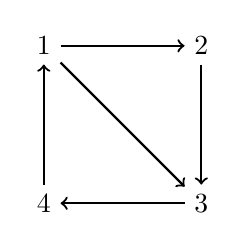
\begin{tikzpicture}
\node (atom1) at (0,2) {1};
\node (atom2) at (2,2) {2};
\node (atom3) at (2,0) {3};
\node (atom4) at (0,0) {4};
\draw[->, thick] (atom1)--(atom2);
\draw[->, thick] (atom2)--(atom3);
\draw[->, thick] (atom3)--(atom4);
\draw[->, thick] (atom4)--(atom1);
\draw[->, thick] (atom1) -- (atom3);
\end{tikzpicture}
\end{center}
Dieses Diagramm könnten wir nutzen, um eine Interpretation zu beschreiben, deren Domäne die ersten vier natürlichen Zahlen sind und `$\atom{R}{x,y}$' so interpretiert, dass es auf und nur auf
	\begin{center}
		\ntuple{1, 2}, 
		\ntuple{2, 3}, 
		\ntuple{3, 4}, 
		\ntuple{4, 1}, 
		\ntuple{1, 3}
	\end{center}
zutrifft. Gleichfalls könnten wir dieses Diagramm anbieten:
\begin{center}
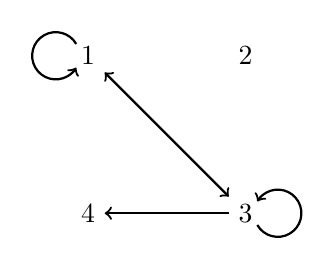
\begin{tikzpicture}
\node (atom1) at (0,2) {1};
\node (atom2) at (2,2) {2};
\node (atom3) at (2,0) {3};
\node (atom4) at (0,0) {4};
\draw[->, thick] (atom3)--(atom4);
\draw[->, thick] (atom1)+(-0.15,0.15) arc (-330:-30:.3); 
\draw[->, thick] (atom3)+(0.15,-0.15) arc (-150:150:.3); 
\draw[<->, thick] (atom1) -- (atom3);
\end{tikzpicture}
\end{center}
um eine Interpretation mit der gleichen Domäne darzustellen, welche allerdings die Extension von `$\atom{R}{x,y}$' wie folgt bestimmt:
	\begin{center}
		\ntuple{1, 3}, 
		\ntuple{3, 1}, 
		\ntuple{3, 4}, 
		\ntuple{1, 1},
		\ntuple{3, 3}
	\end{center}
Wenn wir wollten, könnten wir unsere Diagramme komplexer gestalten. Zum Beispiel könnten wir Namen als Beschriftungen für bestimmte Objekte hinzufügen. Gleicherma{\ss}en könnten wir, um die Extension eines einstelligen Prädikats zu symbolisieren, einfach einen Kreis um bestimmte Objekte zeichnen und festlegen, dass das Prädikat `$\atom{H}{x}$' auf die so eingekreisten Objekte (und nur sie) zutrifft. 

\chapter{Wahrheit in der LEO}\label{s:TruthFOL}
Da Interpretationen uns unter anderem sagen, welche Prädikate auf welche Objekte zutreffen, bestimmen sie, welche atomaren Sätze wahr und welche falsch sind. Nun müssen wir aber genau sagen, was es bedeutet, wenn ein willkürlicher LEO-Satz in einer Interpretation wahr oder falsch ist. 

Wir wissen dank \S\ref{s:FOLSentences}, dass es drei verschiedene Arten von Sätzen in der LEO gibt: 
	\begin{ebullet}
		\item atomare Sätze
		\item Sätze, deren Hauptoperator ein Junktor ist
		\item Sätze, deren Hauptoperator ein Quantor ist
	\end{ebullet}
Wir müssen getrennt erklären, was es bedeutet, wenn solche Sätze wahr oder falsch sind.

Um unsere Erklärung verständlich zu machen, werden wir immer wieder die folgende Interpretation verwenden:
	\begin{ekey}
		\item[\text{Domäne}] Alle Personen, die vor 2000 geboren wurden
		\item[a] Aristoteles
		\item[b] Beyonc\'e
		\item[\atom{P}{x}] \gap{x} ist Philosoph*in
		\item[\atom{R}{x,y}] \gap{x} wurde vor \gap{y} geboren
	\end{ekey}

\section{atomare Sätze}
Die Wahrheit atomarer Sätze ist recht einfach zu erklären. Für Satzbuchstaben gilt: die Interpretation legt fest, welche wahr und welche falsch sind. Der Satz `$\atom{P}{a}$' ist wahr genau dann, wenn `$\atom{P}{x}$' auf `$a$' zutrifft. Unserer Interpretation nach, ist das der Fall, genau dann, wenn Aristoteles Philosoph ist. Das ist der Fall. Also ist der Satz wahr. Gleichfalls ist `$\atom{P}{b}$' unserer Interpretation nach falsch.

Ähnlicherweise ist `$\atom{R}{a,b}$' unserer Interpretation nach wahr genau dann, wenn das Objekt, auf das `$a$' verweist, vor dem Objekt, das `$b$' benennt, geboren wurde. Da Aristoteles vor Beyonc\'e geboren wurde ist `$\atom{R}{a,b}$' wahr. Gleichfalls ist `$\atom{R}{a,a}$' falsch: Aristoteles wurde nicht vor Aristoteles geboren. 

Die Wahrheit atomarer Sätze zu erklären ist also recht einfach. Wenn \metav{R} ein $n$-stelliges Prädikat ist and $\metav{a}_1$, $\metav{a}_{2}$, \dots, $\metav{a}_{n}$ Namen sind, dann gilt:

	\factoidbox{
		Der Satz $\atom{\metav{R}}{\metav{a}_{1},\metav{a}_{2},\dots,\metav{a}_{n}}$ ist einer Interpretation nach wahr genau dann, wenn $\metav{R}$ in dieser Interpretation auf die von $\metav{a}_{1}$, $\metav{a}_{2}$, \dots, $\metav{a}_{n}$ benannten Objekte (in dieser Reihenfolge) zutrifft.
	}

Es gibt auch noch eine spezielle Art von atomarem Satz: zwei Namen, die mittels des Identitätssymbols verbunden wurden. Die Wahrheit solcher Sätze ist auch einfach zu erklären. Wenn \metav{a} und \metav{b} beliebige Namen sind, dann gilt: 
	\factoidbox{
		$\metav{a} = \metav{b}$ ist einer Interpretation nach wahr genau dann, wenn $\metav{a}$ und $\metav{b}$ in dieser Interpretation dasselbe Objekt benennen.
	}
In unserer Beispielinterpretation ist also `$a = b$' falsch, weil Aristoteles von Beyonc\'e verschieden ist.

\section{Junktoren}
In \S\ref{s:FOLSentences} sahen wir, dass in der LEO, wie in der WFL, Sätze mittels der Junktoren aus Basiselementen gebaut werden können. Die Regeln für diese Junktoren sind \emph{genau} die gleichen, wie im Fall der WFL. Hier sind sie:
	\factoidbox{
		$\metav{A} \eand \metav{B}$ ist in einer Interpretation wahr genau dann, wenn sowohl $\metav{A}$ als auch $\metav{B}$ in dieser Interpretation wahr sind.
		
		\medskip
		
		$\metav{A} \eor \metav{B}$ ist in einer Interpretation wahr genau dann, wenn in dieser Interpretation entweder $\metav{A}$ wahr ist oder $\metav{B}$ wahr ist.

		\medskip
		
		$\enot \metav{A}$ ist in einer Interpretation wahr genau dann, wenn $\metav{A}$ falsch ist in dieser Interpretation.

		\medskip
		
		$\metav{A} \eif \metav{B}$ ist in einer Interpretation wahr genau dann, wenn in dieser Interpretation entweder $\metav{A}$ falsch ist oder $\metav{B}$ wahr ist.

		\medskip
		
		$\metav{A} \eiff \metav{B}$ ist in einer Interpretation wahr genau dann, wenn in dieser Interpetation $\metav{A}$ den gleichen Wahrheitswert wie $\metav{B}$ hat.
	}
Diese Tabelle stellt die gleiche Informationen wie die charakteristischen Wahrheitstabellen für die Junktoren dar, nur auf eine etwas andere Weise. Einige Beispiele werden dazu beitragen, die Idee zu veranschaulichen. In unserer Beispielinterpretation gilt:
	\begin{earg}
		\item[\textbullet] `$a = a \eand \atom{P}{a}$' ist wahr
		\item[\textbullet] `$\atom{R}{a,b} \eand \atom{P}{b}$' ist falsch, denn, obwohl `$\atom{R}{a,b}$' wahr ist, ist `$\atom{P}{b}$' falsch
		\item[\textbullet] `$a = b \eor \atom{P}{a}$' ist wahr
		\item[\textbullet] `$\enot a = b$' ist wahr
		\item[\textbullet] `$\atom{P}{a} \eand \enot( a= b \eand \atom{R}{a,b})$' ist wahr, weil `$\atom{P}{a}$' wahr ist und `$a = b$' falsch
	\end{earg}

\section{Quantoren}\label{s:MainLogicalOperatorQuantifier}
Die aufregende Neuerung der LEO ist die Verwendung von \emph{Quantoren}. Aber die Wahrheitsbedingungen für quantifizierte Sätze auszudrücken ist kniffliger, als man zunächst erwarten würde. 

Hier ist ein na\"{i}ver erster Gedanke. Wir wollen sagen, dass `$\forall x\, \atom{F}{x}$' wahr ist genau dann, wenn `$\atom{F}{x}$' auf alle Objekte in der Domäne zutrifft. Das sollte nicht problematisch sein: denn unsere Interpretation bestimmt ja, auf was `$\atom{F}{x}$' zutrifft. 

Leider ist dieser na\"{i}ve Gedanke nicht allgemein genug. Wir wollen zum Beispiel sagen könnnen, dass `$\forall x \exists y\, \atom{L}{x,y}$' wahr ist genau dann, wenn (ungefähr) `$\exists y\, \atom{L}{x,y}$' auf alles in der Domäne zutrifft. Aber unsere Interpretation bestimmt nicht \emph{direkt} auf was `$\exists y\, \atom{L}{x,y}$' zutrifft. Doch, ob dies auf etwas zutrifft oder nicht, sollte sich allein aus der Interpretation des Prädikats `$L$', der Domäne und der Bedeutung der Quantoren ergeben.

Hier ist also ein zweiter na\"{i}ver Gedanke. Wir versuchen nun zu sagen, dass `$\forall x \exists y\, \atom{L}{x,y}$' in einer Intepretation wahr ist genau dann, wenn $\exists y\, \atom{L}{\metav{a},y}$ für \emph{jeden} Namen \metav{a}, den wir in unserer Interpretation auflisten, wahr ist. Ähnlicherweise versuchen wir nun zu sagen, dass $\exists y\, \atom{L}{\metav{a},y}$ wahr ist genau dann, wenn $\atom{L}{\metav{a},\metav{b}}$ für \emph{zumindest einen} Namen \metav{b}, den wir in unserer Interpretation aufgelistet haben, wahr ist.

Leider funktioniert auch das nicht. Beachten Sie, dass unsere Interpretation nur \emph{zwei} Namen, $a$ und $b$ auflistet. Aber die Domäne--alle Personen, die vor dem Jahr 2000 geboren wurden--umfasst viel mehr als zwei Personen. (Und wir haben nicht die Absicht, dies zu korrigieren, indem wir versuchen, alle mit Namen auszustatten.)

Hier ist also ein dritter Gedanke. (Dieser Gedanke ist nicht na\"{i}v, sondern richtig.) Obwohl es nicht der Fall ist, dass wir jedes einzelne Objekt benannt haben, \emph{hätte} jeder Person ein Name gegeben werden können. Wir sollten uns also auf die Möglichkeit konzentrieren, eine Interpretation durch Hinzufügen eines neuen Namens zu erweitern. Wir werden einige Beispiele dafür geben, wie dies funktioniert, wobei wir uns auf unsere Beispielinterpretation konzentrieren werden. Danach stellen wir die entsprechende formale Definition vor. 

In unserer Beispielinterpretation sollte `$\exists x\, \atom{R}{b,x}$' wahr sein. Denn in der Domäne gibt es mit Sicherheit jemanden, der nach Beyonc\'e geboren wurde. Lady Gaga zum Beispiel. Falls wir unsere Beispielinterpretation erweitern würden---nur kurzfristig natürlich---indem wir bestimmen, dass der Name `$c$' Lady Gaga benennt, dann wäre `$\atom{R}{b,c}$' in dieser erweiterten Interpretation wahr. Das macht `$\exists x\, \atom{R}{b,x}$' laut unserer ursprünglichen Interpretation wahr.

In unserer Beispielinterpretation sollte auch `$\exists x (\atom{P}{x} \eand \atom{R}{x,a})$' wahr sein. Denn in unserer Domäne gibt es sicherlich jemanden, die sowohl Philosoph*in war und vor Aristoteles geboren wurde. Sokrates zum Beispiel. Wenn wir unsere Beispielinterpretation erweitern würden, und `$c$' als Name für Sokrates verwendeten, dann wäre `$\atom{W}{c} \eand \atom{R}{c,a}$' in dieser erweiterten Interpretation wahr. Das macht `$\exists x (\atom{P}{x} \eand \atom{R}{x,a})$' laut unserer ursprünglichen Interpretation wahr. 
%Gendern ist hier Geschmackssache.. 

Ein letztes Beispiel: `$\forall x \exists y\, \atom{R}{x,y}$' sollte in unserer Beispielinterpretation falsch sein. Denn wir wissen zwar nicht, wer die letzte Person ist, die 1999 geboren wurde, aber es gibt sie. Und wenn wir unsere Beispielinterpretation erweitern, und `$d$' als Namen für diese Person verwenden würden, dann wären wir nicht in der Lage, eine weitere Person zu finden, die wir mit einem weiteren Namen benennen könnten, und die nach $d$ geboren wurde. Egal wen wir mit einem weiteren Namen, z.B.\@ `$e$', benennen täten, `$\atom{R}{d,e}$' wäre falsch. Das macht `$\exists y\, \atom{R}{d,y}$' \emph{falsch} in unserer erweiterten Interpretation. Und das wiederum macht `$\forall x \exists y\, \atom{R}{x,y}$' falsch, laut unserer ursprünglichen Interpretation.

Diese drei Beispiele geben uns einen Startpunkt für unsere formale Definition der Wahrheit von Sätzen, deren Hauptoperatoren Quantoren sind. Diese Definition erfordert aber leider einiges an Arbeit.

Nehmen Sie an, dass \metav{A} eine Formel ist, die zumindest ein Vorkommnis der Variable \metav{x} enthält, und, dass $\metav{x}$ in $\metav{A}$ ungebunden ist. Wir fassen dies so zusammen:
$$\metav{A}(\ldots \metav{x} \ldots \metav{x} \ldots)$$
Nehmen Sie auch an, dass \metav{c} ein Name ist. Nun schreiben wir:
$$\metav{A}(\ldots \metav{c} \ldots \metav{c} \ldots)$$
um die Formel zu symbolisieren, die wir erhalten, wenn wir \emph{jedes} Vorkommnis von $\metav{x}$ in \metav{A} mit $\metav{c}$ ersetzen. Die resultierende Formel nennen wir eine \define{Substitutionsinstanz} von $\forall \metav{x}\metav{A}$ und $\exists\metav{x}\metav{A}$. Dementsprechend nennen wir $\metav{c}$ den \define{substituierenden Namen}. Also gilt:
	$$\exists x (\atom{R}{e,x} \eiff \atom{F}{x})$$
ist eine Substitutionsinstanz von 
	$$\forall y \exists x (\atom{R}{y,x} \eiff \atom{F}{x})$$
dessen substituierender Name `$e$', und substituierte Variable `$y$', ist.

\newglossaryentry{substitution instance}{
  name = Substitutionsinstanz,
  description = {Das Resultat des Ersetzens jedes ungebundenen Vorkommnisses einer \gls{Variable} in einer \gls{Formel} mit einem \gls{Name}n}
}

Unsere Interpretation beinhaltet eine Bestimmung dazu, welche Objekte in der Domäne welchen Namen entsprechen. Nehmen Sie nun ein beliebiges Objekt der Domäne, $d$ beispielsweise, und einen Namen $\metav{c}$, der nicht schon in unserer Interpretation genutzt wird. Wenn unsere Interpretation $\mathbf{I}$ ist, dann können wir uns nun mit der Interpretation $\mathbf{I}[d/\metav{c}]$ beschäftigen, die $\mathbf{I}$ genau entspricht, au{\ss}er, dass sie \emph{auch} den Namen $\metav{c}$ dem Objekt $d$ zuordnet. Nun können wir sagen, dass $d$ die Formel $\metav{A}(\dots\metav{x}\dots\metav{x}\dots)$ in Interpretation $\mathbf{I}$ \define{erfüllt} genau dann, wenn $\metav{A}(\dots\metav{c}\dots\metav{c}\dots)$ in $\mathbf{I}[d/\metav{c}]$ wahr ist. (Wenn $d$ $\metav{A}(\dots\metav{x}\dots\metav{x}\dots)$ erfüllt, dann sagen wir auch, dass $\metav{A}(\dots\metav{x}\dots\metav{x}\dots)$ auf $d$ zutrifft.) 

\factoidbox{Die Interpretation $\mathbf{I}[d/\metav{c}]$ entspricht $\mathbf{I}$ genau, au{\ss}er, dass sie dem Objekt $d$ den Namen $\metav{c}$ zuordnet.

\
\\

Ein Objekt $d$ \define{erfüllt} $\metav{A}(\dots\metav{x}\dots\metav{x}\dots)$ in $\mathbf{I}$ genau dann, wenn $\metav{A}(\dots\metav{c}\dots\metav{c}\dots)$ in $\mathbf{I}[d/\metav{c}]$ wahr ist.
}

Zum Beispiel erfüllt Sokrates die Formel $\atom{P}{x}$, weil $\atom{P}{c}$ in der Interpretation $\mathbf{I}[\text{Sokrates}/c]$ wahr ist (hier ist die Interpretation):
\begin{ekey}
	\item[\text{Domäne}] Alle Personen, die vor 2000 geboren wurden
	\item[a] Aristoteles
	\item[b] Beyonc\'e
	\item[c] Sokrates 
	\item[\atom{P}{x}] \gap{x} ist Philosoph*in
	\item[\atom{R}{x,y}] \gap{x} wurde vor \gap{y} geboren
\end{ekey}

Mit all diesen Definitionen bewaffnet lautet die grobe Idee wie folgt. Der Satz $\forall \metav{x}\metav{A}(\ldots \metav{x} \ldots \metav{x} \ldots)$ ist in $\mathbf{I}$ wahr genau dann, wenn für jedes Objekt $d$ in der Domäne gilt, dass $\metav{A}(\ldots \metav{c} \ldots \metav{c}\ldots)$ in $\mathbf{I}[d/\metav{c}]$ wahr ist (egal welches Objekt in der Domäne wir mit $\metav{c}$ benennen). Anders ausgedrückt: $\forall \metav{x} \metav{A}(\ldots \metav{x} \ldots \metav{x} \ldots)$ ist wahr genau dann, wenn jedes Objekt in der Domäne $\metav{A}(\ldots \metav{x} \ldots \metav{x} \ldots)$ erfüllt. Ähnlicherweise ist der Satz $\exists \metav{x}\metav{A}(\ldots \metav{x} \ldots \metav{x} \ldots)$ wahr genau dann, wenn es \emph{zumindest ein Objekt} gibt, das $\metav{A}(\ldots \metav{x} \ldots \metav{x} \ldots)$ erfüllt (d.h.\@ wenn $\metav{A}(\ldots \metav{c} \ldots \metav{c} \ldots)$ in $\mathbf{I}[d/\metav{c}]$ für zumindest ein Objekt $d$ wahr ist).
	\factoidbox{
		$\forall \metav{x}\metav{A}(\ldots \metav{x}\ldots\metav{x}\ldots)$ ist wahr in einer Interpretation genau dann, wenn jedes Objekt in der Domäne $\metav{A}(\ldots \metav{x} \ldots \metav{x}\ldots)$ erfüllt.
		\
		\\
		
		$\exists \metav{x}\metav{A}(\ldots \metav{x}\ldots\metav{x}\ldots)$ ist wahr in einer Interpretation genau dann, wenn zumindest ein Objekt in der Domäne
		$\metav{A}(\ldots \metav{x}\ldots\metav{x}\ldots)$ erfüllt.
	}
All das hier formalisiert die intuitive Idee, die wir vorher schon ausgedrückt hatten. Das Resultat ist leider weder elegant noch allzu einfach verständlich. 

Lasst uns zuletzt noch betonen, dass der Begriff eines Objekts, das eine Formel mit einer ungebundenen Variable erfüllt, auch auf Formeln mit mehr als einer ungebundenen Variable ausgedehnt werden kann. Wenn wir eine Formel $\metav{A}(\metav{x},\metav{y})$ mit zwei ungebundenen Variablen $\metav{x}$ and $\metav{y}$ haben, dann können wir sagen, dass ein Objektpaar $\langle a, b\rangle$ $\metav{A}(\metav{x},\metav{y})$ erfüllt genau dann, wenn $\metav{A}(\metav{c},\metav{d})$ in der Interpretation, die wir mit zwei Namen $\metav{c}$ und $\metav{d}$ für $a$ und $b$ erweitert haben, wahr ist. Beispielsweise erfüllt $\langle \text{Sokrates}, \text{Plato}\rangle$ $R(x,y)$, da $R(c,d)$ laut der folgenden Interpretation wahr ist:
\begin{ekey}
	\item[\text{Domäne}] Alle Personen, die vor 2000 geboren wurden
	\item[a] Aristoteles
	\item[b] Beyonc\'e
	\item[c] Sokrates
	\item[d] Plato
	\item[\atom{P}{x}] \gap{x} ist Philosoph*in
	\item[\atom{R}{x,y}] \gap{x} wurde vor \gap{y} geboren
\end{ekey}
Für atomare Formeln sind die Objekte, Objektpaare, etc.\@ die sie erfüllen, genau jene, die in die angegebene Extension ihrer Prädikate fallen. Aber der Begriff der Erfüllung findet auch auf nicht-atomare Formeln Anwendung. Die Formel $\atom{P}{x} \land \atom{R}{x,b}$ wird zum Beispiel von allen Philosoph*innen, die vor Beyonc\'e geboren wurden, erfüllt. Der Begriff findet sogar auf quantifizierte Formeln Anwendung. $P(x) \eand \lnot\exists y(P(y) \land R(y,x))$ zum Beispiel wird von allen Personen, die Philosoph*innen sind, erfüllt; und von solchen, vor denen kein*e einzige Philosoph*in geboren wurde, erfüllt.

\practiceproblems
\problempart
\label{pr.TorF1}
Betrachten Sie die folgende Interpretation:
	\begin{ebullet}
		\item Domäne: Fatih und Benedikt
		\item `$\atom{A}{x}$' trifft auf Fatih und Benedikt zu
		\item `$\atom{B}{x}$' trifft nur auf Benedikt zu
		\item `$\atom{N}{x}$' trifft auf niemanden zu.
		\item `$f$' verweist auf Fatih
	\end{ebullet}
Bestimmen Sie, ob die folgenden Sätze in dieser Interpretation wahr oder falsch sind.
\begin{earg}
\item $\atom{B}{f} $
\item $\atom{A}{f}  \eiff \enot \atom{N}{f}$
\item $\atom{N}{f}  \eif (\atom{A}{f} \eor \atom{B}{f})$
\item $\forall x\, \atom{A}{x}$
\item $\forall x \enot \atom{B}{x}$
\item $\exists x(\atom{A}{x} \eand \atom{B}{x})$
\item $\exists x(\atom{A}{x} \eif \atom{N}{x})$
\item $\forall x(\atom{N}{x} \eor \enot \atom{N}{x})$
\item $\exists x\, \atom{B}{x} \eif \forall x\, \atom{A}{x}$
\end{earg}

\problempart
\label{pr.TorF2}
Betrachten Sie die folgende Interpretation:
	\begin{ebullet}
		\item Domäne: Lemmy, Courtney und Eddy
		\item `$\atom{G}{x}$' trifft auf Lemmy, Courtney und Eddy zu.
		\item `$\atom{H}{x}$' trifft nur auf Courtney zu.
		\item `$\atom{M}{x}$' trifft nur auf Lemmy und Eddy zu.
		\item `$c$' verweist auf Courtney
		\item `$e$' verweist auf Eddy
	\end{ebullet}
Bestimmen Sie, ob die folgenden Sätze in dieser Interpretation wahr oder falsch sind.
\begin{earg}
\item $\atom{H}{c} $
\item $\atom{H}{e} $
\item $\atom{M}{c}  \eor \atom{M}{e}$
\item $\atom{G}{c}  \eor \enot \atom{G}{c}$
\item $\atom{M}{c}  \eif \atom{G}{c}$
\item $\exists x\, \atom{H}{x}$
\item $\forall x\, \atom{H}{x}$
\item $\exists x\, \enot \atom{M}{x}$
\item $\exists x(\atom{H}{x} \eand \atom{G}{x})$
\item $\exists x(\atom{M}{x} \eand \atom{G}{x})$
\item $\forall x(\atom{H}{x} \eor \atom{M}{x})$
\item $\exists x\, \atom{H}{x} \eand \exists x\, \atom{M}{x}$
\item $\forall x(\atom{H}{x} \eiff \enot \atom{M}{x})$
\item $\exists x\, \atom{G}{x} \eand \exists x \enot \atom{G}{x}$
\item $\forall x\exists y(\atom{G}{x} \eand \atom{H}{y})$
\end{earg}

\problempart
\label{pr.TorF3}
Betrachten Sie die folgende diagrammatisch dargestellte Interpretation:
\begin{center}
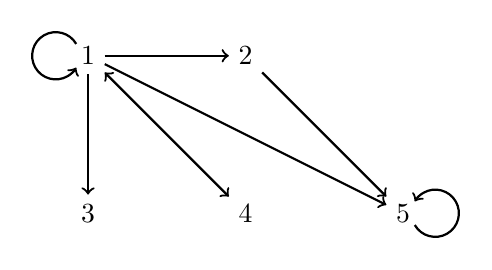
\begin{tikzpicture}
\node (atom1) at (0,2) {1};
\node (atom2) at (2,2) {2};
\node (atom4) at (0,0) {3};
\node (atom5) at (2,0) {4};
\node (atom6) at (4,0) {5};
\draw[->, thick] (atom1)+(-0.15,0.15) arc (-330:-30:.3); 
\draw[->, thick] (atom6)+(0.15,-0.15) arc (-150:150:.3); 
\draw[->, thick] (atom1) -- (atom2);
\draw[->, thick] (atom1) -- (atom4);
\draw[<->, thick] (atom1) -- (atom5);
\draw[->, thick] (atom1) -- (atom6);
\draw[->, thick] (atom2) -- (atom6);
\end{tikzpicture}
\end{center}
($\atom{R}{x,y}$ trifft auf $x$ und $y$ (in dieser Reihenfolge) zu genau dann, wenn ein Pfeil von x auf y zeigt.) Bestimmen Sie, ob die folgenden Sätze in dieser Interpretation wahr oder falsch sind.
\begin{earg}
\item $\exists x\, \atom{R}{x,x}$
\item $\forall x\, \atom{R}{x,x}$
\item $\exists x \forall y\, \atom{R}{x,y}$
\item $\exists x \forall y\, \atom{R}{y,x}$
\item $\forall x \forall y \forall z ((\atom{R}{x,y} \eand \atom{R}{y,z}) \eif \atom{R}{x,z})$
\item $\forall x \forall y \forall z ((\atom{R}{x,y} \eand \atom{R}{x,z}) \eif \atom{R}{y,z})$
\item $\exists x \forall y\, \enot \atom{R}{x,y}$
\item $\forall x(\exists y\, \atom{R}{x,y} \eif \exists y\, \atom{R}{y,x})$
\item $\exists x \exists y (\enot x = y \eand \atom{R}{x,y} \eand \atom{R}{y,x})$
\item $\exists x \forall y(\atom{R}{x,y} \eiff x = y)$
\item $\exists x \forall y(\atom{R}{y,x} \eiff x = y)$
\item $\exists x \exists y(\enot x = y \eand \atom{R}{x,y} \eand \forall z(\atom{R}{z,x} \eiff y = z))$
\end{earg}


\chapter{Semantische Begriffe}

Die Wahrheit in der LEO zu definieren war sehr aufwändig. Aber nun, da wir das getan haben, können wir eine Reihe anderer Begriffe definieren. Unsere Definitionen werden denen der WFL, in \S\ref{s:SemanticConcepts}, sehr ähneln. Allerdings berufen sie sich auf \emph{Interpretationen} anstelle von Bewertungen. 

Das Symbol `$\entails$' nutzen wir auch in der LEO:
	$$\metav{A}_1, \metav{A}_2, \ldots, \metav{A}_n \entails\metav{C}$$
bedeutet, dass es keine Interpretation gibt, in der $\metav{A}_1$, $\metav{A}_2$, \dots, $\metav{A}_n$ alle wahr sind und \metav{C} falsch ist. Dementsprechend bedeutet
	$$\entails\metav{A}$$
dass \metav{A} in jeder Interpretation wahr ist.

Die anderen logischen Begriffe haben entsprechende Definitionen:

\begin{itemize}
\item Ein LEO-Satz $\metav{A}$ ist eine \define{Tautologie} genau dann, wenn $\metav{A}$ in jeder Interpretation wahr ist, d.h.\@ $\entails\metav{A}$.
\newglossaryentry{validity}
{
name=Tautologie (der LEO),
description={Ein \gls{Satz der LEO}, der in jeder \gls{Interpretation} wahr ist}
}

\item $\metav{A}$ ist ein \define{Widerspruch} genau dann, wenn $\metav{A}$ in jeder Interpretation falsch ist; d.h.\@ $\entails\enot\metav{A}$.
\newglossaryentry{contradiction of FOL}
{
  name=Widerspruch (der LEO),
  text=Widerspruch,
description={Ein \gls{Satz der LEO}, der in jeder \gls{Interpretation} falsch ist}
}
  
\item $\metav{A}_1, \metav{A}_2, \ldots \metav{A}_n \therefore \metav{C}$ ist \define{gültig in der LEO} genau dann, wenn es keine Interpretation gibt, in der die Prämissen wahr sind und die Schlussfolgerung falsch; d.h.\@, $\metav{A}_1,\metav{A}_2,\ldots \metav{A}_n \entails\metav{C}$. Andernfalls ist es \define{ungültig in der LEO}.
\newglossaryentry{valid in FOL}
{
  name=Gültigkeit von Argumenten (in der LEO),
  text = gültig,
description={Eine Eigenschaft von Argumenten, laut der keine \gls{interpretation} die Prämissen wahr und die Schlussfolgerung falsch macht}
}

\item Zwei LEO-Sätze \metav{A} und \metav{B} sind \define{äquivalent} genau dann, wenn sie in genau den gleichen Interpretation wahr sind; d.h.\@ $\metav{A}\entails\metav{B}$ und $\metav{B}\entails\metav{A}$.

\newglossaryentry{equivalent in FOL}
{
  name=Äquivalenz (in der LEO),
  text = äquivalent,
description={Eine Eigenschaft von zwei Sätzen der LEO, laut der die Sätze in jeder \gls{Interpretation} den gleichen Wahrheitswert haben}
}

\item Die LEO-Sätze $\metav{A}_1$, $\metav{A}_2$, \dots, $\metav{A}_n$ sind \define{konsistent} genau dann, wenn zumindest eine Interpretation beide wahr macht. Sie sind \define{inkonsistent} genau dann, wenn es keine solche Interpretation gibt.
\newglossaryentry{satisfiable in FOL}
{
  name=Konsistenz (in der LEO),
  text=konsistent,
description={Eine Eigenschaft von Sätzen der LEO, laut der diese Sätze in zumindest einer \gls{Interpretation} gemeinsam wahr sind}
}
\end{itemize}

\chapter{Interpretationen nutzen}
\label{sec.UsingModels}

\section{Tautologien und Widersprüche}
Nehmen wir an, wir wollen zeigen, dass `$\exists x\, \atom{A}{x,x} \eif \atom{B}{d}$' keine Tautologie ist. Dazu müssen wir zeigen, dass der Satz nicht in allen Interpretation wahr ist, d.h.\@, dass er in zumindest einer Interpretation falsch ist. Wenn wir eine Interpretation liefern, in der der Satz falsch ist, dann zeigen wir also, dass er keine Tautologie ist.

Damit `$\exists x\,\atom{A}{x,x} \eif \atom{B}{d}$' falsch ist, muss sein Antezedens (`$\exists x\, \atom{A}{x,x}$') wahr sein und das Konsequens (`$\atom{B}{d}$') falsch. Um eine entsprechende Interpretation zu konstruieren, starten wir mit einer Domäne. Die Domäne klein zu halten hilft beim Bestimmen der Extensionen der Prädikate. Also beginnen wir mit einer Domäne mit nur einem Element: die Stadt Paris. 
	\begin{ekey}
		\item[\text{Domäne}] Paris
	\end{ekey}
Der Name `$d$' muss auf etwas in der Domäne verweisen:
	\begin{ekey}
		\item[d] Paris
	\end{ekey}
Wir wollen nun, dass `$\exists x\, \atom{A}{x,x}$' wahr ist. Also wollen wir, dass alle Elemente der Domäne mit sich selbst in der Extension von `$A$' gepaart werden. Das erreichen wir hiermit:
	\begin{ekey}
		\item[\atom{A}{x,y}] \gap{x} ist identisch zu \gap{y}
	\end{ekey}
Jetzt ist `$\atom{A}{d,d}$' wahr und auch `$\exists x\, \atom{A}{x,x}$'. Nun wollen wir, dass `$\atom{B}{d}$' falsch ist. Also darf der Referent von `$d$' nicht in der Extension von `$B$' sein. Das erreichen wir so:
	\begin{ekey}
		\item[\atom{B}{x}] \gap{x} ist in Deutschland
	\end{ekey}
Schon haben wir eine Interpretation, in der `$\exists x\, \atom{A}{x,x}$' wahr ist, aber `$\atom{B}{d}$' falsch. Also gibt es eine Interpretation, in der `$\exists x\, \atom{A}{x,x} \eif \atom{B}{d}$' falsch ist. `$\exists x\, \atom{A}{x,x} \eif \atom{B}{d}$' ist keine Tautologie.

Genauso einfach können wir zeigen, dass `$\exists x\atom{A}{x,x} \eif \atom{B}{d}$' kein Widerspruch ist. Wir brauchen nur eine Interpretation, in der `$\exists x\atom{A}{x,x} \eif \atom{B}{d}$' wahr ist, d.h.\@ eine Interpretation, in der entweder `$\exists x\, \atom{A}{x,x}$' falsch ist oder `$\atom{B}{d}$' wahr ist. Hier ist eine:
	\begin{ekey}
		\item[\text{Domäne}] Paris
		\item[d] Paris
		\item[\atom{A}{x,y}] \gap{x} ist identisch mit \gap{y}
		\item[\atom{B}{x}] \gap{x} ist in Frankreich
	\end{ekey}
Das zeigt, dass es zumindest eine Interpretation gibt, in der `$\exists x\atom{A}{x,x} \eif \atom{B}{d}$' wahr ist. `$\exists x\, \atom{A}{x,x} \eif \atom{B}{d}$' ist also kein Widerspruch.
	\factoidbox{
		Um zu zeigen, dass $\metav{A}$ keine Tautologie ist, reicht es, eine Interpretation zu finden, in der $\metav{A}$ falsch ist.
		
		Um zu zeigen, dass $\metav{A}$ kein Widerspruch ist, reicht es, eine Interpretation zu finden, in der $\metav{A}$ wahr ist.
	}

\section{Äquivalenz}
Nehmen wir an, wir wollen zeigen, dass `$\forall x\, \atom{S}{x}$' und `$\exists x\, \atom{S}{x}$' nicht äquivalent sind. Dazu brauchen wir eine Interpretation, in der die zwei Sätze verschiedene Wahrheitswerte haben; einer muss wahr, der andere falsch sein. Wir beginnen mit einer Domäne. Auch hier halten wir die Domäne möglichst klein. Aber hier brauchen wir zumindest zwei Objekte. (In einer Domäne mit nur einem Element haben die Sätze den gleichen Wahrheitswert. Um das zu sehen, versuche, ein paar Interpretation mit nur einem Element zu konstruieren.) Lasst uns die Domäne so ``befüllen'':
	\begin{ekey}
		\item[\text{Domäne}] Ornette Coleman, Miles Davis
	\end{ekey}
`$\exists x\, \atom{S}{x}$' machen wir wahr, indem wir etwas zur Extension von `$S$' hinzufügen und `$\forall x\, \atom{S}{x}$' machen wir falsch, indem wir etwas aus der Extension au{\ss}en vor lassen. Zum Beispiel:
	\begin{ekey}
		\item[\atom{S}{x}] \gap{x} spielt Saxophon
	\end{ekey}
Jetzt ist `$\exists x\, \atom{S}{x}$' wahr, weil `$\atom{S}{x}$' auf Ornette Coleman zutrifft. Präziser gesagt: erweitern wir unsere Interpretation, indem wir `$c$' auf Ornette Coleman verweisen lassen. `$\atom{S}{c}$' ist in dieser erweiterten Interpretation wahr. Also ist `$\exists x\, \atom{S}{x}$' in unserer ursprünglichen Interpretation wahr. Ähnlicherweise ist `$\forall x\, \atom{S}{x}$' falsch, da `$\atom{S}{x}$' nicht auf Miles Davis zutrifft. Genauer gesagt: Wir erweitern unsere Interpretation, indem wir `$d$' auf Miles Davis verweisen lassen. `$\atom{S}{d}$' ist in dieser erweiterten Interpretation falsch. Also ist `$\forall x\, \atom{S}{x}$' in unserer ursprünglichen Interpretation falsch. Wir haben eine \emph{Gegeninterpretation} zur Aussage, dass `$\forall x\, \atom{S}{x}$' und `$\exists x\, \atom{S}{x}$' äquivalent sind geliefert.
	\factoidbox{
		Um zu zeigen, dass $\metav{A}$ und $\metav{B}$ nicht äquivalent sind, reicht es, eine Intepretation zu finden, in der einer der beiden Sätze wahr ist, der andere aber falsch.
	}

\section{Gültigkeit, Folge und Konsistenz}
Um auf Gültigkeit, Folge und Konsistenz zu testen, brauchen wir normalerweise Intepretationen, welche die Wahrheitswerte von mehreren Sätzen bestimmen. 

Betrachten Sie das folgende Argument der LEO:
$$\exists x(\atom{G}{x} \eif \atom{G}{a}) \therefore \exists x\, \atom{G}{x} \eif \atom{G}{a}$$
Um zu zeigen, dass dieses Argument ungültig ist, müssen wir die Prämisse wahr und die Schlussfolgerung falsch machen. Die Schlussfolgerung ist ein Konditional. Um sie falsch zu machen, muss daher ihr Antezedens wahr und ihr Konsequens falsch sein. Unsere Domäne muss hierzu zumindest zwei Objekte beinhalten. Lasst es uns mit folgender Interpretation versuchen:
	\begin{ekey}
		\item[\text{Domäne}] Karl Marx, Ludwig von Mises
		\item[\atom{G}{x}] \gap{x} hasste den Kommunismus
		\item[a] Karl Marx
	\end{ekey}
Da Marx \emph{das kommunistische Manifest} schrieb, ist `$\atom{G}{a}$' in dieser Interpretation klar falsch. Aber von Mises hasste den Kommunismus. Also ist `$\exists x\, \atom{G}{x}$' in dieser Interpretation wahr. Daher ist `$\exists x\, \atom{G}{x} \eif \atom{G}{a}$' falsch, wie benötigt. 

Macht unsere Interpretation die Prämisse unseres Arguments wahr? Ja. `$\atom{G}{a} \eif \atom{G}{a}$' ist wahr, ja sogar eine Tautologie. Aber damit ist `$\exists x (\atom{G}{x} \eif \atom{G}{a})$' wahr. Also ist in dieser Intepretation die Prämisse wahr und die Schlussfolgerung falsch: somit ist das Argument als Ganzes ungültig.

Nebenbei sei darauf hingewiesen, dass `$\exists x(\atom{G}{x} \eif \atom{G}{a})$' nicht `$\exists x\, \atom{G}{x} \eif \atom{G}{a}$' zur Folge hat: $\exists x (\atom{G}{x} \eif \atom{G}{a}) \nentails \exists x \atom{G}{x} \eif \atom{G}{a}$. Damit haben wir gezeigt, dass `$\exists x (\atom{G}{x} \eif \atom{G}{a})$' und `$\enot (\exists x\, \atom{G}{x} \eif \atom{G}{a})$' konsistent sind.

Nehmen wir ein zweites Beispiel her:
$$\forall x \exists y\, \atom{L}{x,y} \therefore \exists y \forall x\, \atom{L}{x,y}$$
Auch hier wollen wir zeigen, dass das Argument ungültig ist. Wir machen hierzu die Prämisse wahr und die Schlussfolgerung falsch. Here ist eine Interpretation:
\begin{ekey}
	\item[\text{Domäne}] Deutsche Bürger*innen, die derzeit in einer Partnerschaft mit genau einem/r anderen deutschen Bürger*in sind
	\item[\atom{L}{x,y}] \gap{x} ist in einer Partnerschaft mit \gap{y}
\end{ekey}
Dieser Interpretation nach ist die Prämisse klarerweise wahr. Alle in der Domäne sind in einer Partnerschaft mit einem/r anderen deutschen Bürger*in. Die andere Bürger*in ist dementsprechend ebenfalls in der Domäne. Für alle in der Domäne gibt es jemand (anders) in der Domäne, mit denen sie in einer Partnerschaft sind. Also ist `$\forall x \exists y\, \atom{L}{x,y}$' wahr. Allerdings ist die Schlussfolgerung klarerweise falsch, denn die Schlussfolgerung bedingt, dass es eine Person gibt, die in einer Partnerschaft mit allen in der Domäne ist. Aber so eine Person gibt es nicht. Das Argument ist also ungültig. 

Nebenbei können wir auch hier direkt beobachten, dass die Sätze `$\forall x \exists y\, \atom{L}{x,y}$' und `$\enot\exists y \forall x\, \atom{L}{x,y}$' konsistent sind und, dass $\forall x \exists y\, \atom{L}{x,y} \nentails \exists y \forall x\, \atom{L}{x,y}$ gilt. 

Für unser drittes Beispiel nutzen wir eine diagrammatische Interpretation:
\begin{center}
	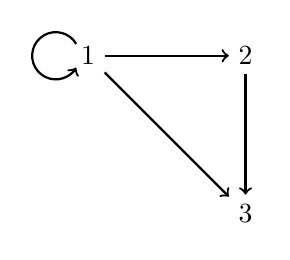
\begin{tikzpicture}
	\node (atom1) at (0,2) {1};
	\node (atom2) at (2,2) {2};
	\node (atom3) at (2,0) {3};
	\draw[->, thick] (atom1)--(atom2);
	\draw[->, thick] (atom1)--(atom3);
	\draw[->, thick] (atom1)+(-0.15,0.15) arc (-330:-30:.3); 
	\draw[->, thick] (atom2) -- (atom3);
	\end{tikzpicture}
\end{center}
Die Domäne dieser Interpretation sind die ersten drei natürlichen Zahlen und `$\atom{R}{x,y}$' trifft auf x und y zu genau dann, wenn es einen Pfeil gibt, der von x zu y zeigt. Hier sind ein paar Sätze, die diese Interpretation wahr machen:
\begin{ebullet}
	\item `$\forall x \exists y\, \atom{R}{y,x}$' 
	\item `$\exists x \forall y\, \atom{R}{x,y}$' \hfill Zeuge 1
	\item `$\exists x \forall y (\atom{R}{y,x} \eiff x = y)$' \hfill Zeuge 1
	\item `$\exists x \exists y \exists z ((\enot y = z \eand \atom{R}{x,y}) \eand \atom{R}{z,x})$' \hfill Zeuge 2
	\item `$\exists x \forall y\, \enot \atom{R}{x,y}$' \hfill Zeuge 3
	\item `$\exists x (\exists y\, \atom{R}{y,x} \eand \enot \exists y\, \atom{R}{x,y})$' \hfill Zeuge 3
\end{ebullet}
Das zeigt uns gleich, dass die obigen sechs Sätze konsistent sind. Wir können diese Beobachtung auch gleich nutzen, um ein paar \emph{ungültige} Argumente zu generieren:
\begin{align*}
	\forall x \exists y\, \atom{R}{y,x}, \exists x \forall y\, \atom{R}{x,y}  &\therefore  \forall x \exists y\, \atom{R}{x,y}\\
	\exists x \forall y\, \atom{R}{x,y}, \exists x \forall y \enot \atom{R}{x,y} & \therefore \enot \exists x \exists y \exists z (\enot y = z \eand (\atom{R}{x,y} \eand \atom{R}{z,x}))
\end{align*}

\factoidbox{
	Wenn eine Interpretation $\metav{A}_1, \metav{A}_2, \ldots, \metav{A}_n$  wahr und $\metav{C}$ falsch macht, dann gilt:
	\begin{ebullet}
		\item$\metav{A}_1, \metav{A}_2, \ldots, \metav{A}_n \therefore \metav{C}$ ist \emph{ungültig}; 
	\item $\metav{A}_1, \metav{A}_2, \ldots, \metav{A}_n \nentails \metav{C}$;
	\item und $\metav{A}_1, \metav{A}_2, \ldots, \metav{A}_n, \enot \metav{C}$ sind konsistent.
\end{ebullet}}
Eine Interpretation, die eine Aussage (dass zwei Sätze konsistent sind, z.B.\@) widerlegt, nennen wir eine \emph{Gegeninterpretation} oder ein \emph{Gegenmodell}. 

Wir beschlie{\ss}en dieses Kapitel mit einer Warnung. Die LEO hat bestimmte Einschränkungen: sie ist eine extensionale Sprache; sie ignoriert vage Eigenschaften; und sie kann Gültigkeit aufgrund ``besonderer Gründe'' nicht einfangen. Als ein Beispiel, nehmen wir dieses Argument her: 
\begin{earg}
	\item[] Alle Männer sind langweilig.
	\item[\therefore] Alle Junggesellen sind langweilig.
\end{earg}
Dies ist ein gültiges Argument: es ist notwendigerweise wahr, dass alle Junggesellen Männer sind. Daher ist es unmöglich, dass die Prämisse wahr ist und die Schlussfolgerung falsch. Nun, könnten wir das Argument versuchen so zu symbolisieren:
$$\forall x(\atom{M}{x} \eif \atom{L}{x}) \therefore \forall x(\atom{J}{x} \eif  \atom{L}{x})$$
Aber es ist einfach, Gegeninterpretationen zu finden, die zeigen, dass $\forall x(\atom{M}{x} \eif \atom{L}{x}) \nentails \forall x(\atom{J}{x} \eif  \atom{L}{x})$. Es wäre aber \emph{falsch} daraus zu schlie{\ss}en, dass das deutsche Argument \emph{ungültig} ist, nur weil es eine Gegeninterpretation zu seiner LEO-Symbolisierung gibt.

\practiceproblems

\problempart
\label{pr.Contingent}
Zeigen Sie, dass die folgenden Sätze weder Tautologien noch Widersprüche sind:
\begin{earg}
\item \leftsolutions\ $\atom{D}{a}  \eand \atom{D}{b}$
\item \leftsolutions\ $\exists x\, \atom{T}{x,h}$
\item \leftsolutions\ $\atom{P}{m}  \eand \enot\forall x\, \atom{P}{x}$
\item $\forall z \atom{J}{z} \eiff \exists y\, \atom{J}{y}$
\item $\forall x (\atom{W}{x,m,n} \eor \exists y\atom{L}{x,y})$
\item $\exists x (\atom{G}{x} \eif \forall y\, \atom{M}{y})$
\item $\exists x (x = h \eand x = i)$
\end{earg}

\solutions
\problempart
\label{pr.NotEquiv}
Zeigen Sie, dass die folgenden Satzpaare nicht äquivalent sind:
\begin{earg}
\item $\atom{J}{a} $,  $\atom{K}{a}$
\item $\exists x\, \atom{J}{x}$,  $\atom{J}{m}$
\item $\forall x\, \atom{R}{x,x}$, $\exists x\, \atom{R}{x,x}$
\item $\exists x\, \atom{P}{x} \eif \atom{Q}{x}$, $\exists x (\atom{P}{x} \eif \atom{Q}{x})$
\item $\forall x(\atom{P}{x} \eif \enot \atom{Q}{x})$, $\exists x(\atom{P}{x} \eand \enot \atom{Q}{x})$
\item $\exists x(\atom{P}{x} \eand \atom{Q}{x})$, $\exists x(\atom{P}{x} \eif \atom{Q}{x})$
\item $\forall x(\atom{P}{x}\eif \atom{Q}{x})$, $\forall x(\atom{P}{x} \eand \atom{Q}{x})$
\item $\forall x\exists y\, \atom{R}{x,y}$, $\exists x\forall y\, \atom{R}{x,y}$
\item $\forall x\exists y\, \atom{R}{x,y}$, $\forall x\exists y\, \atom{R}{y,x}$
\end{earg}



\problempart
Zeigen Sie, dass die folgenden Sätze konsistent sind:
\begin{earg}
\item  $\atom{M}{a}, \enot \atom{N}{a}, \atom{P}{a}, \enot \atom{Q}{a}$
\item $\atom{L}{e,e}, \atom{L}{e,g}, \enot \atom{L}{g,e}, \enot \atom{L}{g,g}$
\item $\enot (\atom{M}{a} \eand \exists x\, \atom{A}{x}), \atom{M}{a} \eor \atom{F}{a}, \forall x(\atom{F}{x} \eif \atom{A}{x})$
\item $\atom{M}{a} \eor \atom{M}{b}, \atom{M}{a} \eif \forall x \enot \atom{M}{x}$
\item $\forall y\, \atom{G}{y}, \forall x (\atom{G}{x} \eif \atom{H}{x}), \exists y \enot \atom{I}{y}$
\item $\exists x(\atom{B}{x} \eor \atom{A}{x}), \forall x \enot \atom{C}{x}, \forall x\bigl[(\atom{A}{x} \eand \atom{B}{x}) \eif \atom{C}{x}\bigr]$
\item $\exists x\, \atom{X}{x}, \exists x\, \atom{Y}{x}, \forall x(\atom{X}{x} \eiff \enot \atom{Y}{x})$
\item $\forall x(\atom{P}{x} \eor \atom{Q}{x}), \exists x\enot(\atom{Q}{x} \eand \atom{P}{x})$
\item $\exists z(\atom{N}{z} \eand \atom{O}{z,z}), \forall x\forall y(\atom{O}{x,y} \eif \atom{O}{y,x})$
\item $\enot \exists x \forall y\, \atom{R}{x,y}, \forall x \exists y\, \atom{R}{x,y}$
\item $\enot \atom{R}{a,a}$, $\forall x (x=a \eor \atom{R}{x,a})$
\item $\forall x\forall y\forall z[(x=y \eor y=z )\eor x=z]$, $\exists x\exists y\ \enot x= y$
\item $\exists x\exists y((\atom{Z}{x} \eand \atom{Z}{y} )\eand x=y)$, $\enot \atom{Z}{d}$, $d=e$
\end{earg}

\problempart
Zeigen Sie, dass die folgenden Argument ungültig sind:
\begin{earg}
\item $\forall x(\atom{A}{x} \eif \atom{B}{x}) \therefore \exists x\, \atom{B}{x}$
\item $\forall x(\atom{R}{x} \eif \atom{D}{x}), \forall x(\atom{R}{x} \eif \atom{F}{x}) \therefore \exists x(\atom{D}{x} \eand \atom{F}{x})$
\item $\exists x(\atom{P}{x}\eif \atom{Q}{x}) \therefore \exists x\, \atom{P}{x}$
\item $\atom{N}{a} \eand \atom{N}{b} \eand \atom{N}{c} \therefore \forall x\, \atom{N}{x}$
\item $\atom{R}{d,e}, \exists x\, \atom{R}{x,d} \therefore \atom{R}{e,d}$
\item $\exists x(\atom{E}{x} \eand \atom{F}{x}), \exists x\, \atom{F}{x} \eif \exists x\, \atom{G}{x} \therefore \exists x(\atom{E}{x} \eand \atom{G}{x})$
\item $\forall x\, \atom{O}{x,c}, \forall x\, \atom{O}{c,x} \therefore \forall x\, \atom{O}{x,x}$
\item $\exists x(\atom{J}{x} \eand \atom{K}{x}), \exists x \enot \atom{K}{x}, \exists x \enot \atom{J}{x} \therefore \exists x(\enot \atom{J}{x} \eand \enot \atom{K}{x})$
\item $\atom{L}{a,b} \eif \forall x\, \atom{L}{x,b}, \exists x\, \atom{L}{x,b} \therefore \atom{L}{b,b}$
\item $\forall x(\atom{D}{x} \eif \exists y\, \atom{T}{y,x}) \therefore \exists y \exists z\ \enot y= z$
\end{earg}

\chapter[Über alle Interpretationen nachdenken]{Über alle Interpretationen nachdenken}

\section{Tautologien und Widersprüche}
Wir können zeigen, dass ein Satz keine Tautologie ist, indem wir nur eine sorgfältig spezifizierte Interpretation liefern: eine Interpretation, in der der Satz falsch ist. Um zu zeigen, dass etwas eine Tautologie ist, reicht es aber nicht aus, zehn, hundert oder sogar tausend Interpretationen zu konstruieren, in denen der Satz wahr ist. Ein Satz ist nur dann eine Tautologie, wenn er in \emph{jeder} Interpretation wahr ist. Aber es gibt unendlich viele Interpretationen. Wir müssen also über sie alle nachdenken. Doch das können wir nicht tun, indem wir uns einzeln mit ihnen befassen!

Manchmal können wir uns recht einfach mit allen Interpretationen befassen. Wir können beispielsweise ein recht einfaches Argument dafür liefern, dass `$\atom{R}{a,a}\eor\enot \atom{R}{a,a}$' eine Tautologie ist:
	\begin{quote}
		\label{allmodels1}
		Jede Interpretation gibt `$\atom{R}{a,a}$' einen Wahrheitswert. Wenn `$\atom{R}{a,a}$' in einer Interpretation wahr ist, dann ist `$\atom{R}{a,a} \eor \enot\atom{R}{a,a}$' in dieser Interpretation wahr. Wenn `$\atom{R}{a,a}$' in einer Interpretation falsch ist, dann ist $\enot\atom{R}{a,a}$ in dieser Interpretation wahr. Damit ist `$\atom{R}{a,a} \eor\enot \atom{R}{a,a}$' in dieser Interpretation wahr. Das sind die einzigen zwei Möglichkeiten. Also ist `$\atom{R}{a,a} \eor\enot \atom{R}{a,a}$' in jeder Interpretation wahr. Dementsprechend ist es eine Tautologie.
	\end{quote}
Dieses Argument ist gültig, aber es ist kein Argument der LEO. Stattdessen ist es ein Argument im Deutschen, unserer Metasprache, das \emph{von} der LEO \emph{handelt}. 

Hier ist eine weitere Eigenschaft dieses Arguments. Weil der Satz, den wir betrachtet haben, keine Quantoren enthielt, mussten wir uns nicht überlegen, wie wir `$a$' und `$R$' interpretieren. Der Punkt war, dass, wie auch immer sie interpretiert werden, `$\atom{R}{a,a}$' den gleichen Wahrheitswert hat.

Sehen wir uns ein weiteres Beispiel an. Der Satz `$\forall x(\atom{R}{x,x}\eor\enot \atom{R}{x,x})$' ist klarerweise eine Tautologie. Doch zu sagen, wieso das so ist stellt sich als schwierig heraus. Wir können nicht sagen, dass `$\atom{R}{x,x} \eor\enot \atom{R}{x,x}$' in jeder Interpretation wahr ist, da `$\atom{R}{x,x} \eor\enot \atom{R}{x,x}$' nicht einmal ein \emph{Satz} der LEO ist (`$x$' ist eine Variable). Stattdessen sollten wir so was sagen:
	\begin{quote}
		Betrachten Sie eine beliebige Interpretation. $\forall x(\atom{R}{x,x}\eor \enot\atom{R}{x,x})$ ist wahr in unserer Interpretation genau dann, wenn $\atom{R}{x,x}\eor\enot\atom{R}{x,x}$ von jedem Objekt in unserer Domäne erfüllt wird. Betrachten Sie nun ein beliebiges Element der Domäne, welches wir Fred nennen. Entweder erfüllt Fred $\atom{R}{x,x}$ oder nicht. Wenn er `$\atom{R}{x,x}$' erfüllt, dann erfüllt Fred auch `$\atom{R}{x,x} \eor \enot \atom{R}{x,x}$'. Wenn Fred `$\atom{R}{x,x}$' nicht erfüllt, erfüllt er \emph{dennoch} `$\enot\atom{R}{x,x}$' und somit auch `$\atom{R}{x,x} \eor\enot \atom{R}{x,x}$'.\footnote{Wir nutzen hier die Tatsache, dass die Wahrheitsbedingungen der Junktoren auch ihre Erfüllungsbedingungen wiederspiegeln: $a$ erfüllt $\metav{A}(\metav{x}) \lor \metav{B}(\metav{x})$ genau dann, wenn $a$ $\metav{A}(\metav{x})$ erfüllt oder $\metav{B}(\metav{x})$ erfüllt, usw.} Wie auch immer, Fred erfüllt `$\atom{R}{x,x} \eor\enot \atom{R}{x,x}$'. Da Fred kein besonderes Element der Domäne war---wir hätten jedes Objekt wählen können---sehen wir, dass jedes Objekt in der Domäne `$\atom{R}{x,x} \eor\enot \atom{R}{x,x}$' erfüllt. Also ist `$\forall x (\atom{R}{x,x} \eor\enot \atom{R}{x,x})$' in unserer Interpretation wahr. Aber wir hatten eine \emph{beliebige} Interpretation gewählt. Daher ist `$\forall x (\atom{R}{x,x} \eor\enot \atom{R}{x,x})$' in jeder Interpretation wahr. Es ist also eine Tautologie.
	\end{quote}
Das alles ist recht langwierig; aber es gibt keine Alternative. Um zu zeigen, dass ein Satz eine Tautologie ist, müssen wir über \emph{alle} Interpretationen nachdenken. 

\section{Andere Fälle}
Ähnliches gilt auch für andere Fälle. Wir müssen über \emph{alle} Interpretationen nachdenken, wenn wir zeigen wollen, dass:
	\begin{ebullet}
		\item ein Satz ein Widerspruch ist, denn dies setzt voraus, dass der Satz in \emph{jeder} Interpretation falsch ist
		\item zwei Sätze äquivalent sind, denn dies setzt voraus, dass sie in \emph{allen} Interpretationen den gleichen Wahrheitswert haben
		\item einige Sätze inkonsistent sind, denn dies setzt voraus, dass es keine Interpretation gibt, in der sie alle wahr sind, d.h.\@, dass in \emph{jeder} Interpretation zumindest einer dieser Sätze falsch ist
		\item ein Argument gültig ist, denn dies setzt voraus, dass die Schlussfolgerung in \emph{allen} Interpretationen wahr ist, in denen die Prämissen wahr sind
		\item einige Sätze einen anderen Satz zur Folge haben.
	\end{ebullet}
Das Problem ist, dass wir mit den bisher vorhandenen Werkzeugen nur schwerlich über alle Interpretationen nachdenken können. Ein letztes Beispiel ist diese Folgebeziehung:
	$$\forall x(\atom{H}{x} \eand \atom{J}{x}) \entails \forall x\, \atom{H}{x}$$
Wenn alle Dinge sowohl $H$ als auch $J$ sind, dann ist alles $H$. Diese Aussage ist also klarerweise wahr. Aber wir können das nur zeigen, indem wir uns ansehen, was in jeder Interpretation, die die Prämisse wahr macht, vor sich geht. Um das zu tun, müssten wir wie folgt argumentieren:
	\begin{quote}
		Betrachten Sie eine beliebige Interpretation in der `$\forall x(\atom{H}{x} \eand \atom{J}{x})$' wahr ist. Es folgt, dass `$\atom{H}{x} \eand \atom{J}{x}$' von allen Objekten dieser Interpretation erfüllt wird. Das aber hei{\ss}t, dass `$\atom{H}{x}$' ebenso von allen Objekten erfüllt wird.\footnote{Hier nutzen wir wieder die Tatsache, dass jedes Objekt welches $\metav{A}(\metav{x}) \land \metav{B}(\metav{x})$ erfüllt, sowohl $\metav{A}(\metav{x})$ als auch $\metav{B}(\metav{x})$ erfüllt.} Also ist `$\forall x\, \atom{H}{x}$' in dieser Interpretation wahr. Wir haben nichts über diese Interpretation angenommen, au{\ss}er, dass sie `$\forall x(\atom{H}{x} \eand \atom{J}{x})$' wahr macht. Also ist jede Interpretation, die `$\forall x(\atom{H}{x} \eand \atom{J}{x})$' wahr macht, eine Interpretation, die auch `$\forall x\, \atom{H}{x}$' wahr macht.
\end{quote}
Selbst für eine einfache Folge wie in unserem Beispiel ist unsere Argumentation recht langwierig. Für kompliziertere Folgen wird die Argumentation entsprechend langwieriger.

Die folgende Tabelle fasst zusammen, ob eine einzelne Interpretation oder Gegeninterpretation ausreicht, oder, ob wir über alle Interpretation nachdenken müssen.

\begin{center}\small
\begin{tabular}{l l l}
%\cline{2-3}
 & \textbf{Yes} & \textbf{No}\\
 \hline
%\cline{2-3}
Tautologie? & alle Interpretationen & eine Gegeninterpretation\\
Widerspruch? &  alle Interpretation  & eine Gegeninterpretation\\
äquivalent? & alle Interpretationen & eine Gegeninterpretation\\
konsistent? & eine interpretation & alle Interpretationen\\
gültig? & alle Interpretationen & eine Gegeninterpretation\\
Folge? & alle Interpretationen & eine Gegeninterpretation\\
\end{tabular}
\end{center}
\label{table.ModelOrArgument}

Es ist vielleicht hilfreich, diese Tabelle mit der in \S\ref{s:PartialTruthTable} zu vergleichen. Der wichtige Unterschied ist, dass die LEO sich mit Interpretationen befasst, während die WFL sich mit Bewertungen befasst. Dieser Unterschied ist wichtig, weil jede Wahrheitstabelle nur endlich viele Zeilen hat, womit eine komplette Wahrheitstabelle ein relativ fügsames Objekt ist. Im Gegensatz dazu gibt es unendlich viele Interpretationen für alle Sätze, was das Nachdenken über alle Interpretationen schwieriger macht. 
